
\section*{Background and Stylised Facts}



\subsection*{Macaronia's Economic Landscape}


In the past decade, the economic development of the \textcolor{teal}{Democratic Republic of Macaronia}, a 
small open economy with a \textcolor{teal}{floating exchange rate} and a population of 4.6 million, was
primarily \textcolor{teal}{FDI-led} and accelerated due to aggressive credit expansion. However, as global 
financial markets fall into turmoil, the country's financial system could face significant risks due to 
domestic vulnerabilities. 

The IMF projects a contraction in \textcolor{teal}{global economic growth} to 2.5\% in 2023 and
3\% in 2024, which is predicted to hit small economies like Macaronia extremely hard.
This  may reduce external investment, increase risks within the financial system, and
 contribute to instability.

Rising \textcolor{teal}{inflation}, heightened tensions in the financial sector, and declining 
\textcolor{teal}{investor confidence} further compound the downside risks to Macaronia’s economy.
A reduction in \textcolor{teal}{foreign capital inflows} could constrain credit conditions and hinder growth. 
If financial stress deepens, reliance on \textcolor{teal}{foreign financing} may expose the country to additional
vulnerabilities, complicating efforts by policymakers to stabilize the economy.

\subsection*{Macaronia's Economic Performance}

% Insert "Real GDP Growth" graph here 
% Insert "Inflation Trends" graph here

\begin{figure}[h]
    \centering
    \begin{subfigure}{0.48\textwidth}
        \centering
        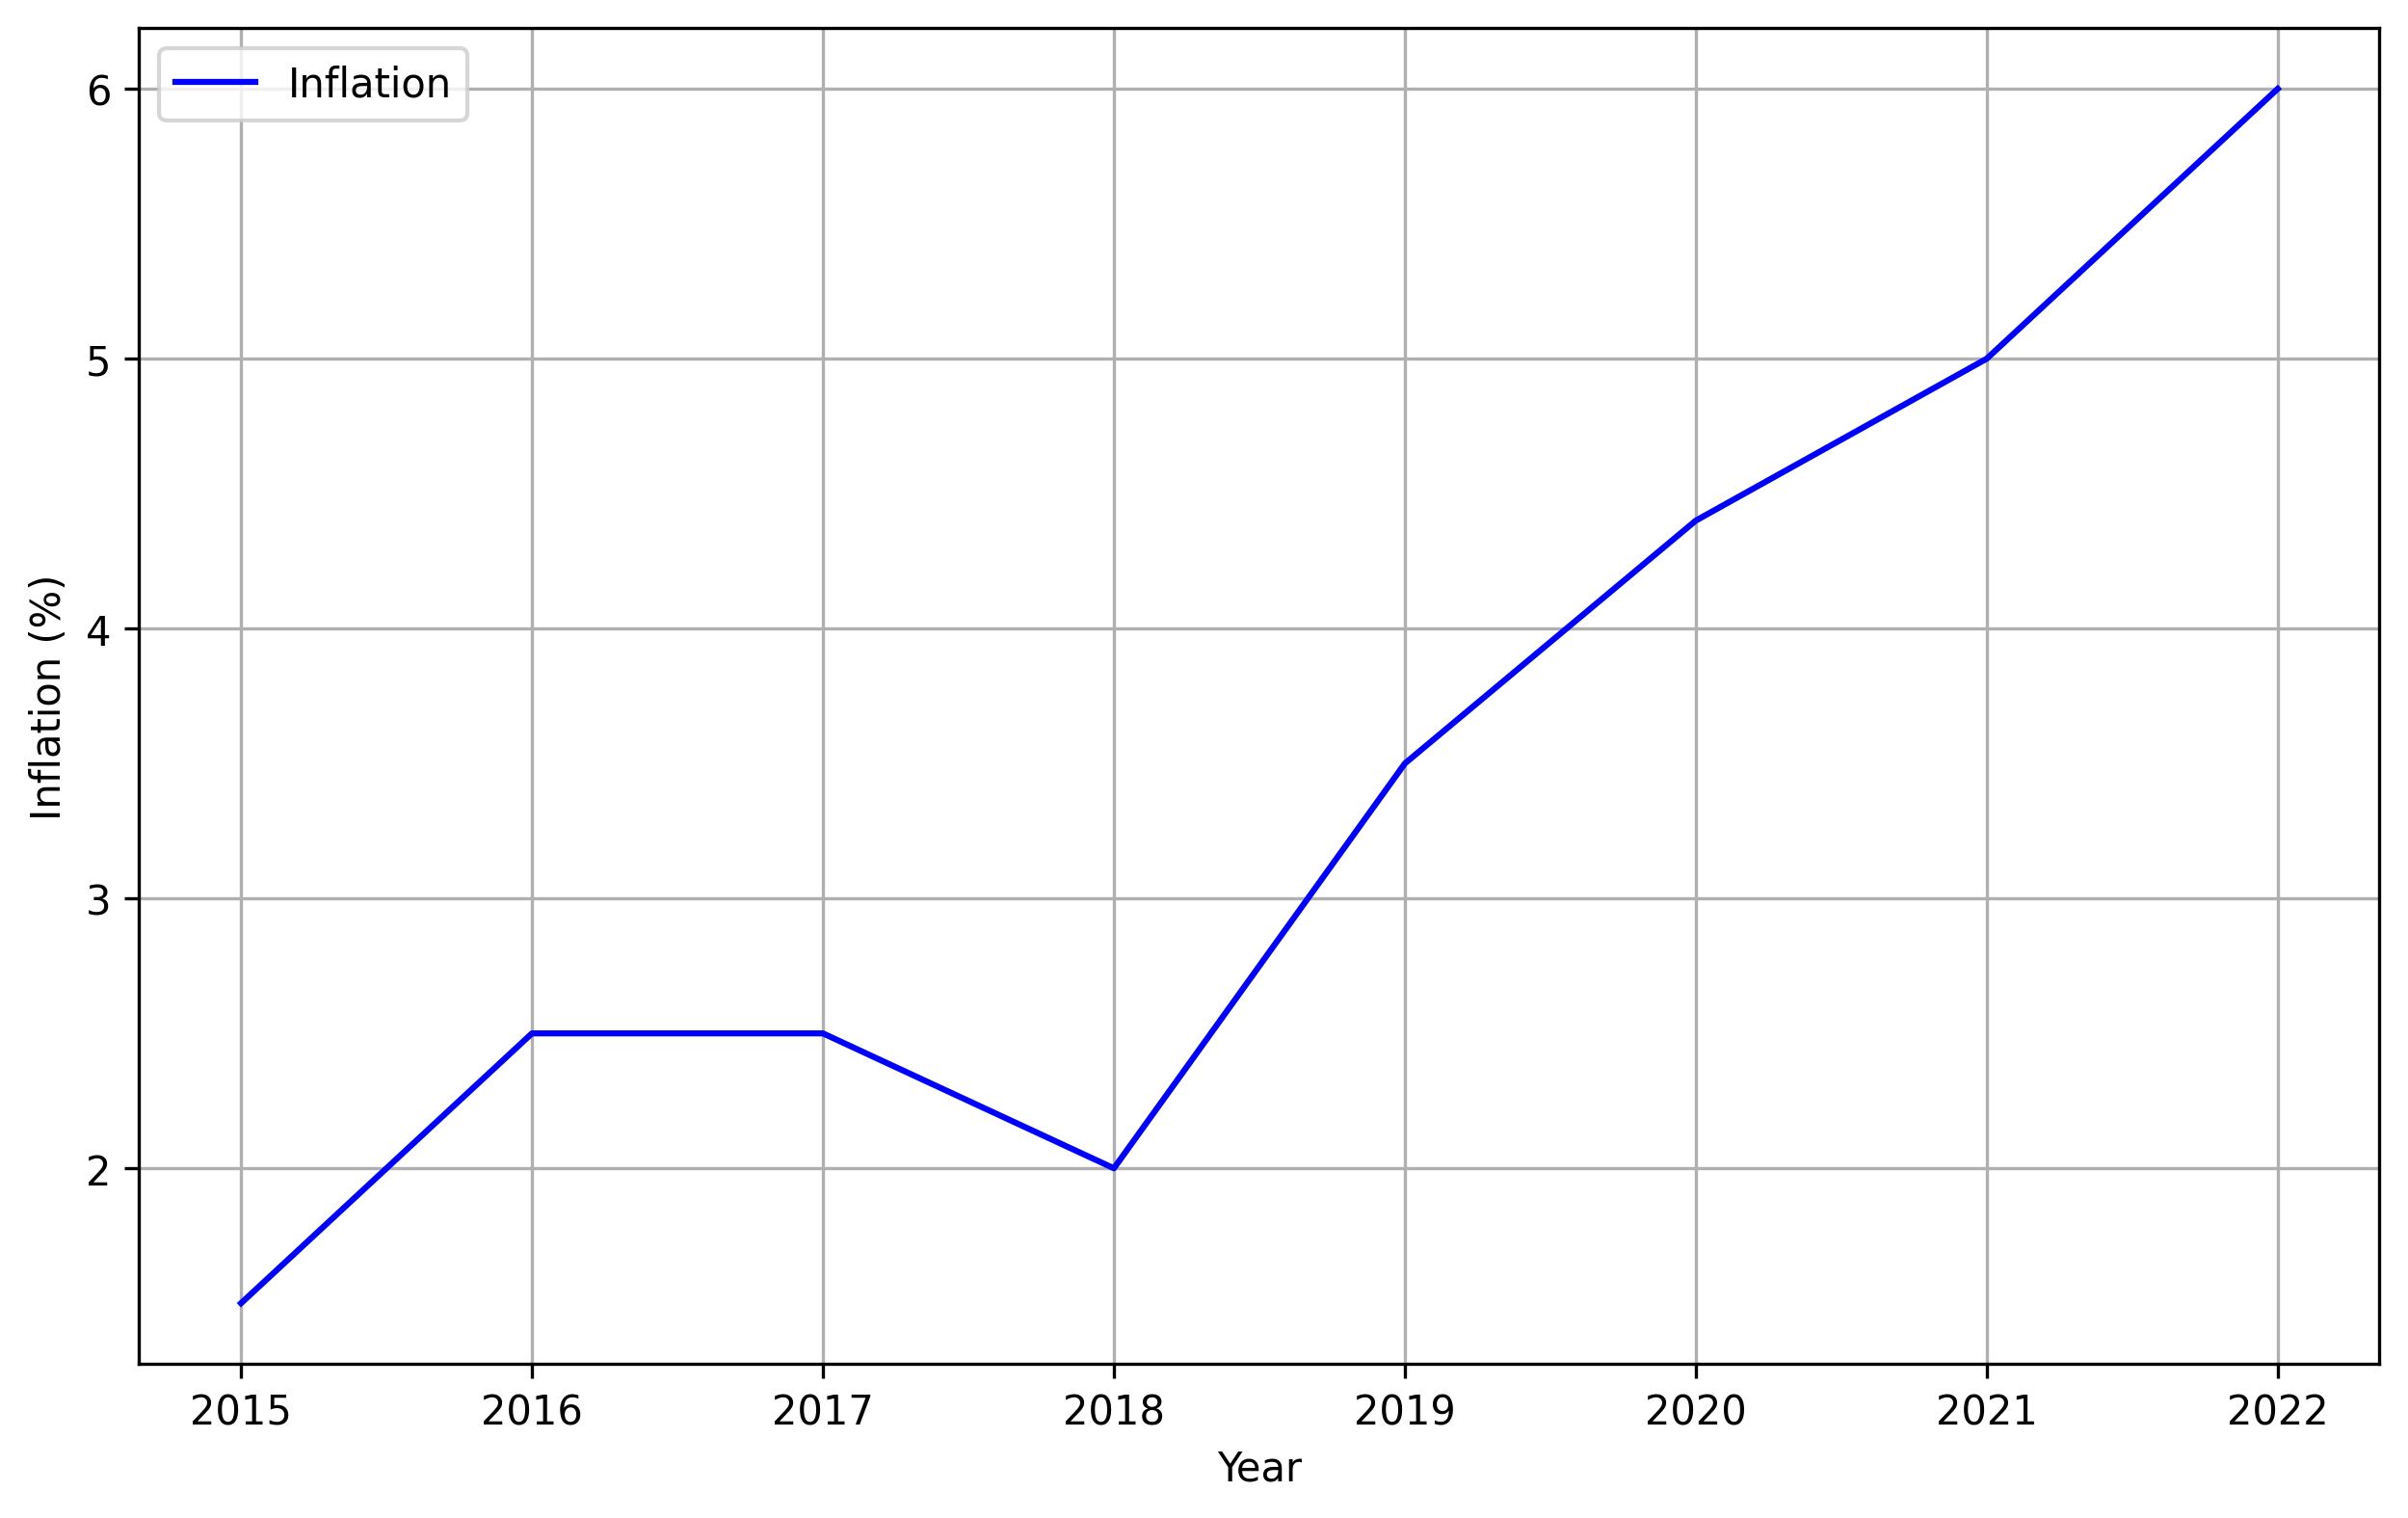
\includegraphics[width=\textwidth]{inflation.png}
        \caption{\small Inflation Rate}
        \label{fig:inflation}
    \end{subfigure}
    \hfill
    \begin{subfigure}{0.48\textwidth}
        \centering
        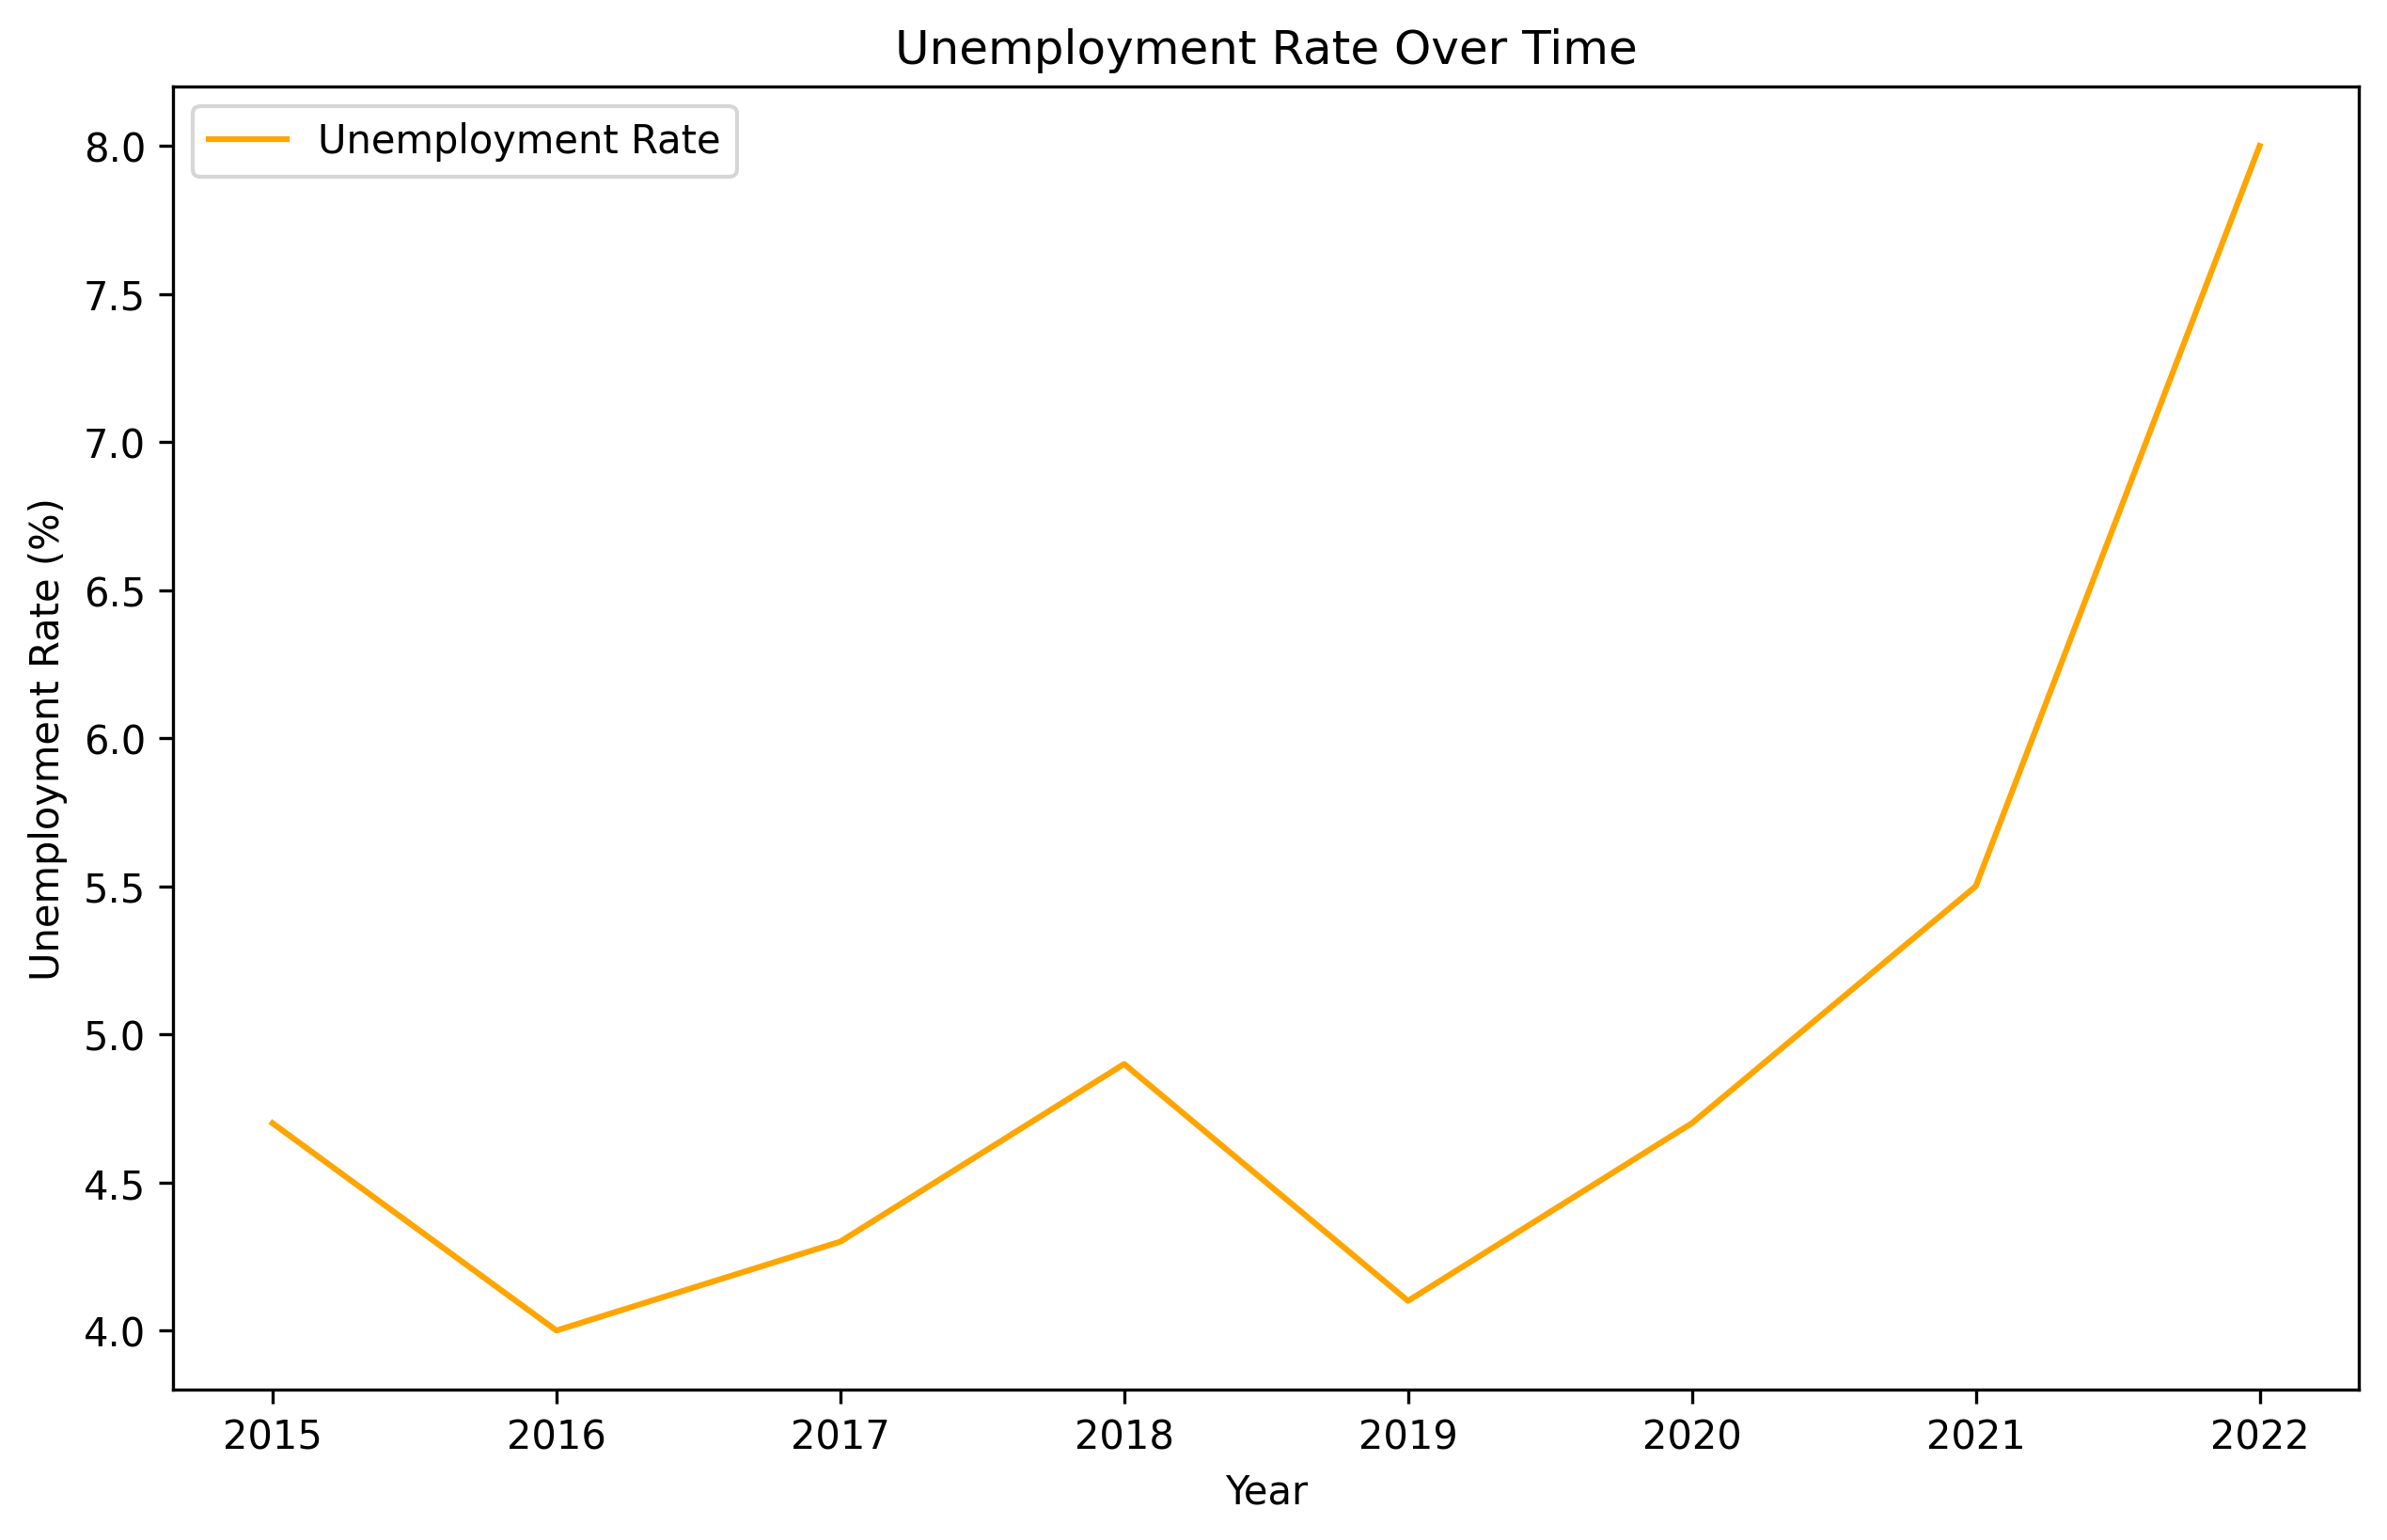
\includegraphics[width=\textwidth]{unemployment.png}
        \caption{\small Unemployment Rate}
        \label{fig:unemployment}
    \end{subfigure}
    \caption{Inflation and Unemployment Trends}  % Main caption for the whole figure
    \label{fig:main_figure}  % Main label for reference
\end{figure}


Macaronia's economy expanded at an average rate of 
\textcolor{teal}{\textbf{4.8\%}}, supported by a booming real estate market. However,
in 2022, the economy contracted by \textcolor{teal}{\textbf{3\%}}, marking the first downturn in nearly a 
decade. The slowdown was mainly driven by the sharp depreciation of REIT values, declining investor confidence,
and tighter global financial conditions.

Figure 1(a) illustrates that inflation rose significantly from \textcolor{teal}{\textbf{1.5\%}}
in 2015 to \textcolor{teal}{\textbf{6\%}} in 2022, fueled by both external price pressures and domestic 
structural vulnerabilities. This surge has been aggravated by the depreciation of the exchange rate and
higher commodity prices, reducing household purchasing power. At the same time, Figure 1(b) demonstrates
that unemployment increased to \textcolor{teal}{\textbf{8\%}} in 2022 from \textcolor{teal}{\textbf{4.7\%}} 
in 2015, as economic activity slowed and businesses reduced hiring. The simultaneous rise 
in \textcolor{teal}{\textbf{inflation}} and \textcolor{teal}{\textbf{unemployment}}, as depicted in
Figures 1(a) and 1(b), suggests that Macaronia is experiencing \textcolor{teal}{\textbf{stagflation}}, 
a challenging economic condition characterized by slow growth, high inflation, and rising unemployment.


\subsection*{Financial Sector Risks and Credit Growth}



Macaronia’s financial system, including commercial banks, credit unions, and insurance companies, 
has expanded greatly in recent years. At the same time, concerns have grown over increasing 
\textcolor{teal}{systemic risks}, especially with excessive exposures to volatile assets like 
\textcolor{teal}{REITs}.  

The commercial banking sector holds assets worth \textcolor{teal}{MCR\$32.0 billion} 
(\textcolor{teal}{20\%} of GDP), with \textcolor{teal}{15\%} of total assets tied up in REITs. 
Credit unions, while smaller, have \textcolor{teal}{MCR\$15.0 billion} in assets, with 
\textcolor{teal}{25\%} of those in REITs.  

The banking sector’s \textcolor{teal}{liquidity position} has weakened, as 
deposit withdrawals have increased in response to concerns about financial stability.
Liquidity ratios dropped from \textcolor{teal}{75\%} in 2020 to \textcolor{teal}{65\%} 
in 2022 for commercial banks, and from \textcolor{teal}{78.8\%} to \textcolor{teal}{68.3\%}
for credit unions. However, \textcolor{teal}{capital adequacy} remains above regulatory benchmarks,
with \textcolor{teal}{12\%} for banks and \textcolor{teal}{10\%} for credit unions.  

These trends align with Diamond and Dybvig’s (1983) model of \textcolor{teal}{bank runs},
which highlights how liquidity mismatches and depositor panic can trigger financial crises. 
The failure of \textcolor{teal}{two} commercial banks in Macaronia due to poor capitalization and
deteriorating asset values underscores these risks.  

\subsection*{Public Sector Debt and Fiscal Position}

\begin{figure}[h]
    \centering
    \begin{subfigure}{0.48\textwidth}
        \centering
        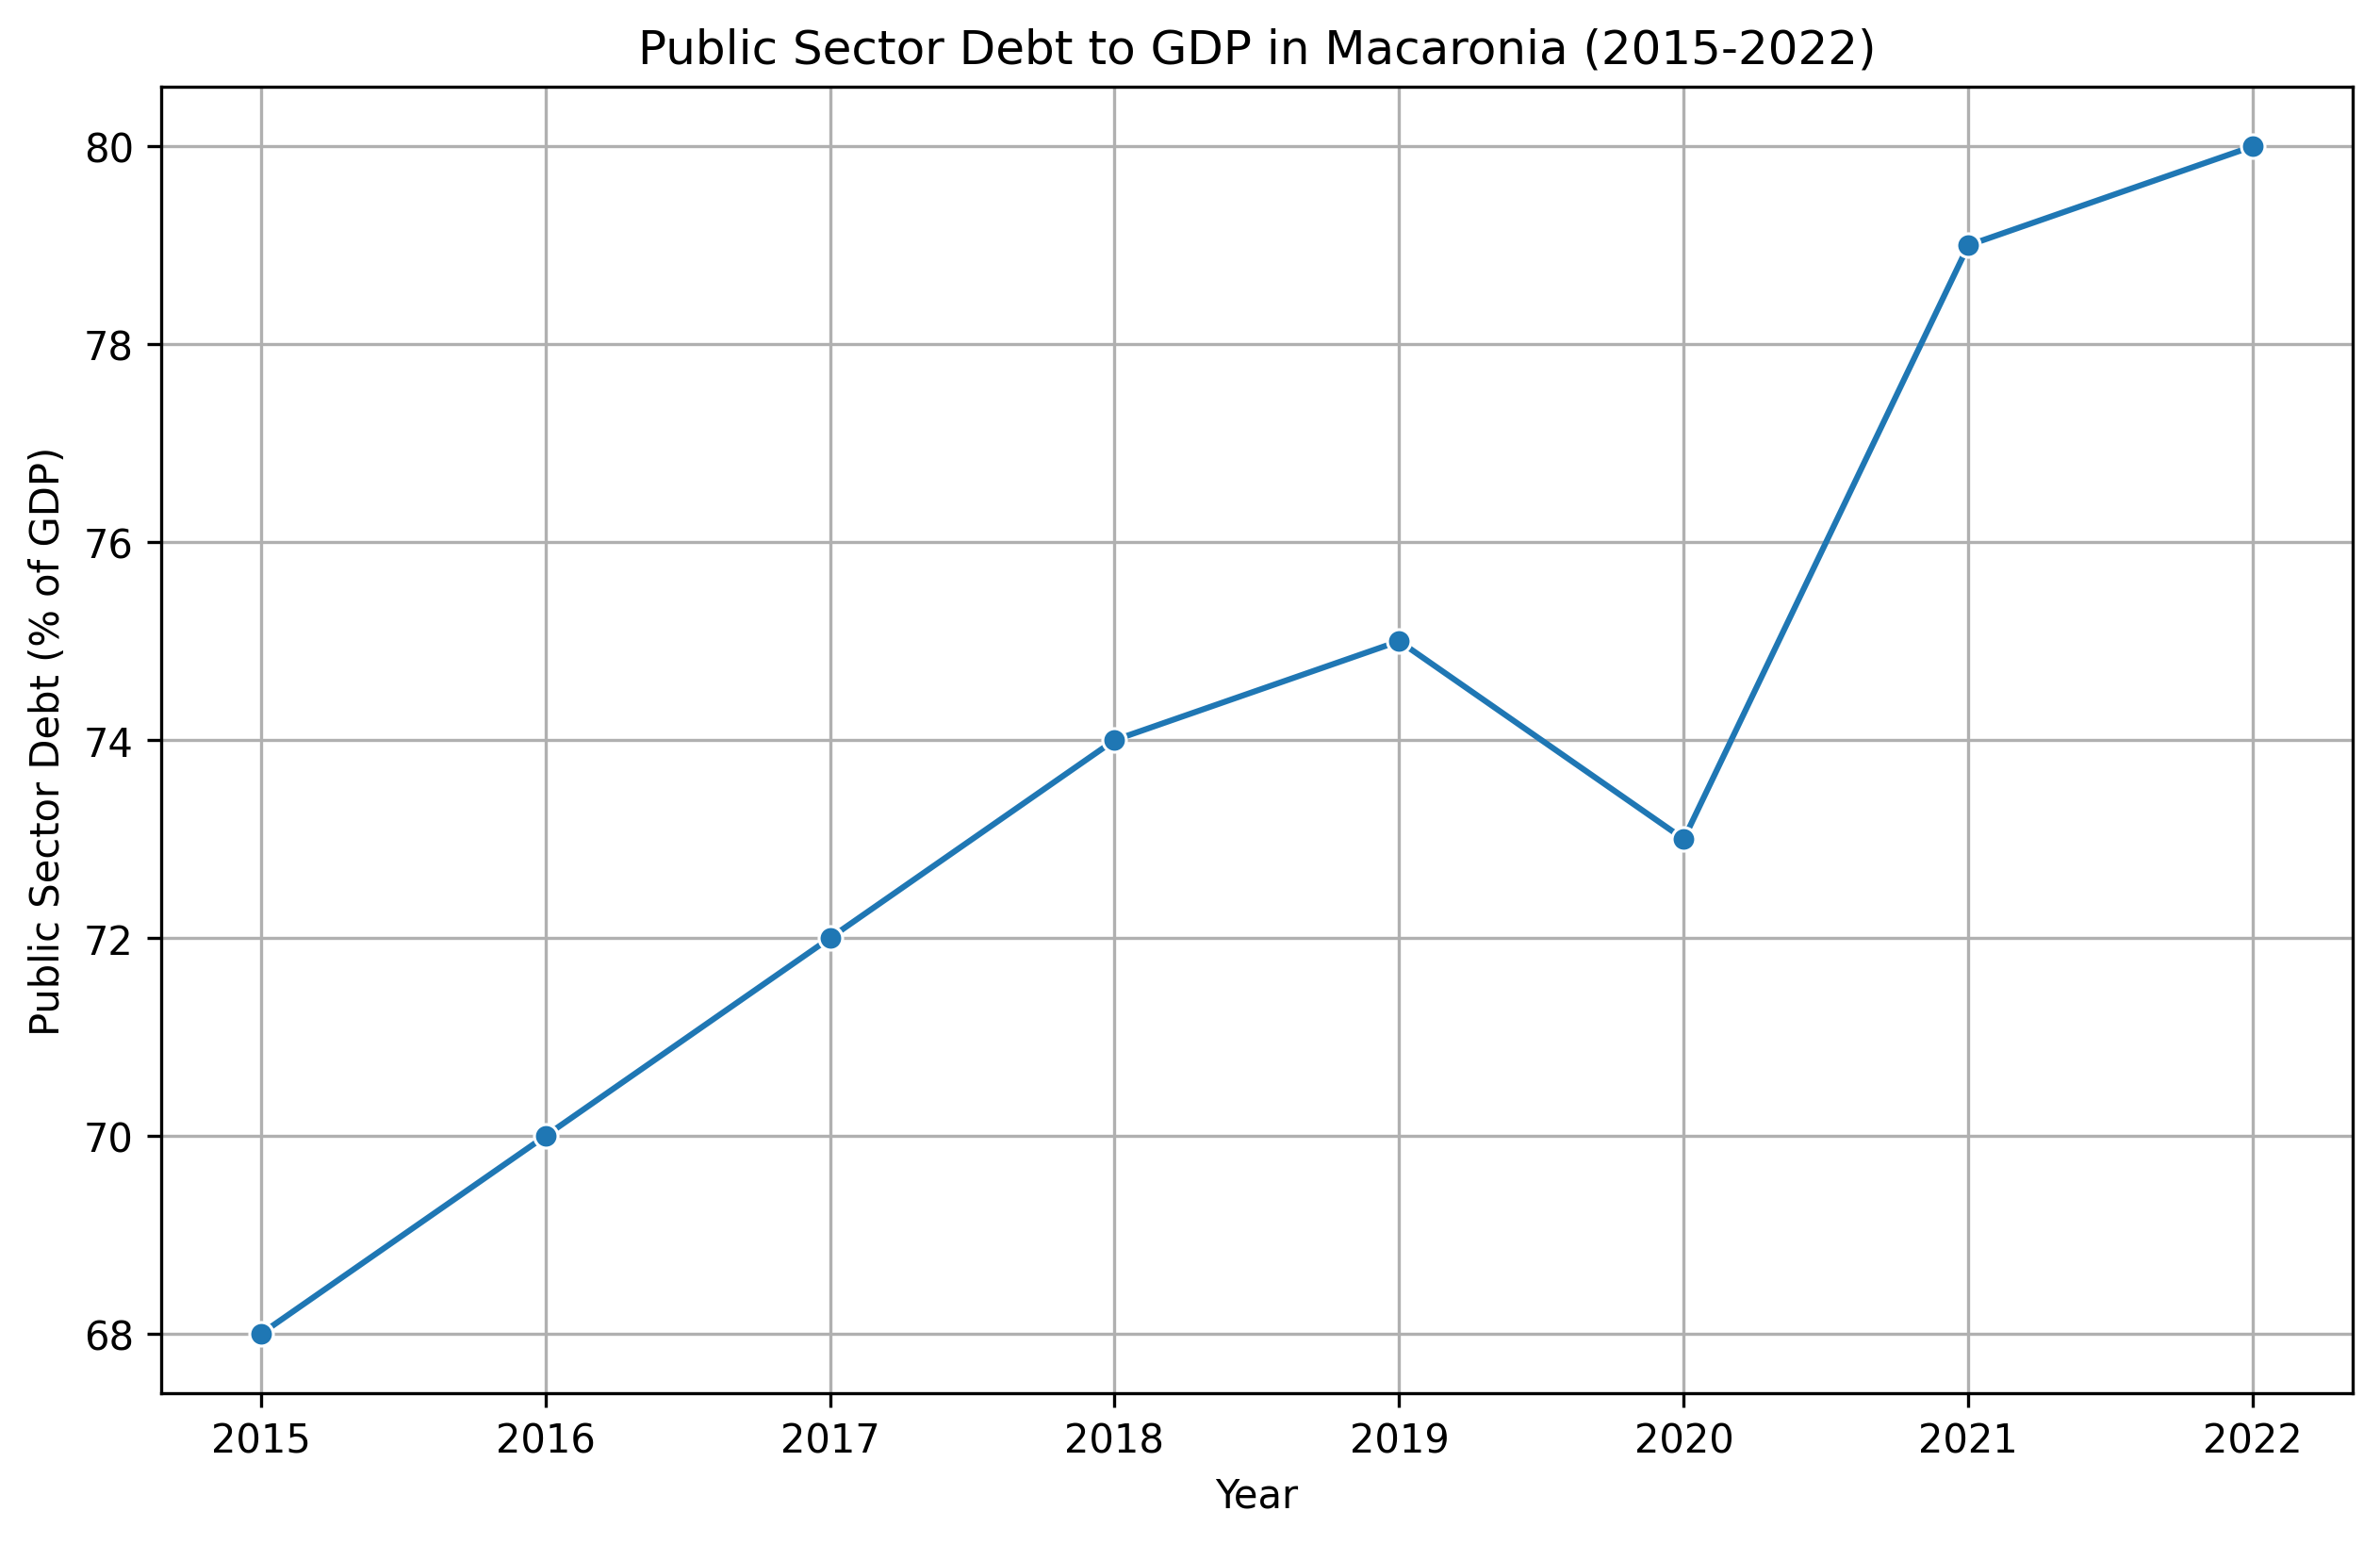
\includegraphics[width=\textwidth]{debt_to_gdp.png}
        \caption{\small Public Sector Debt to GDP in Macaronia}
        \label{fig:debt_to_gdp}
    \end{subfigure}
    \hfill
    \begin{subfigure}{0.48\textwidth}
        \centering
        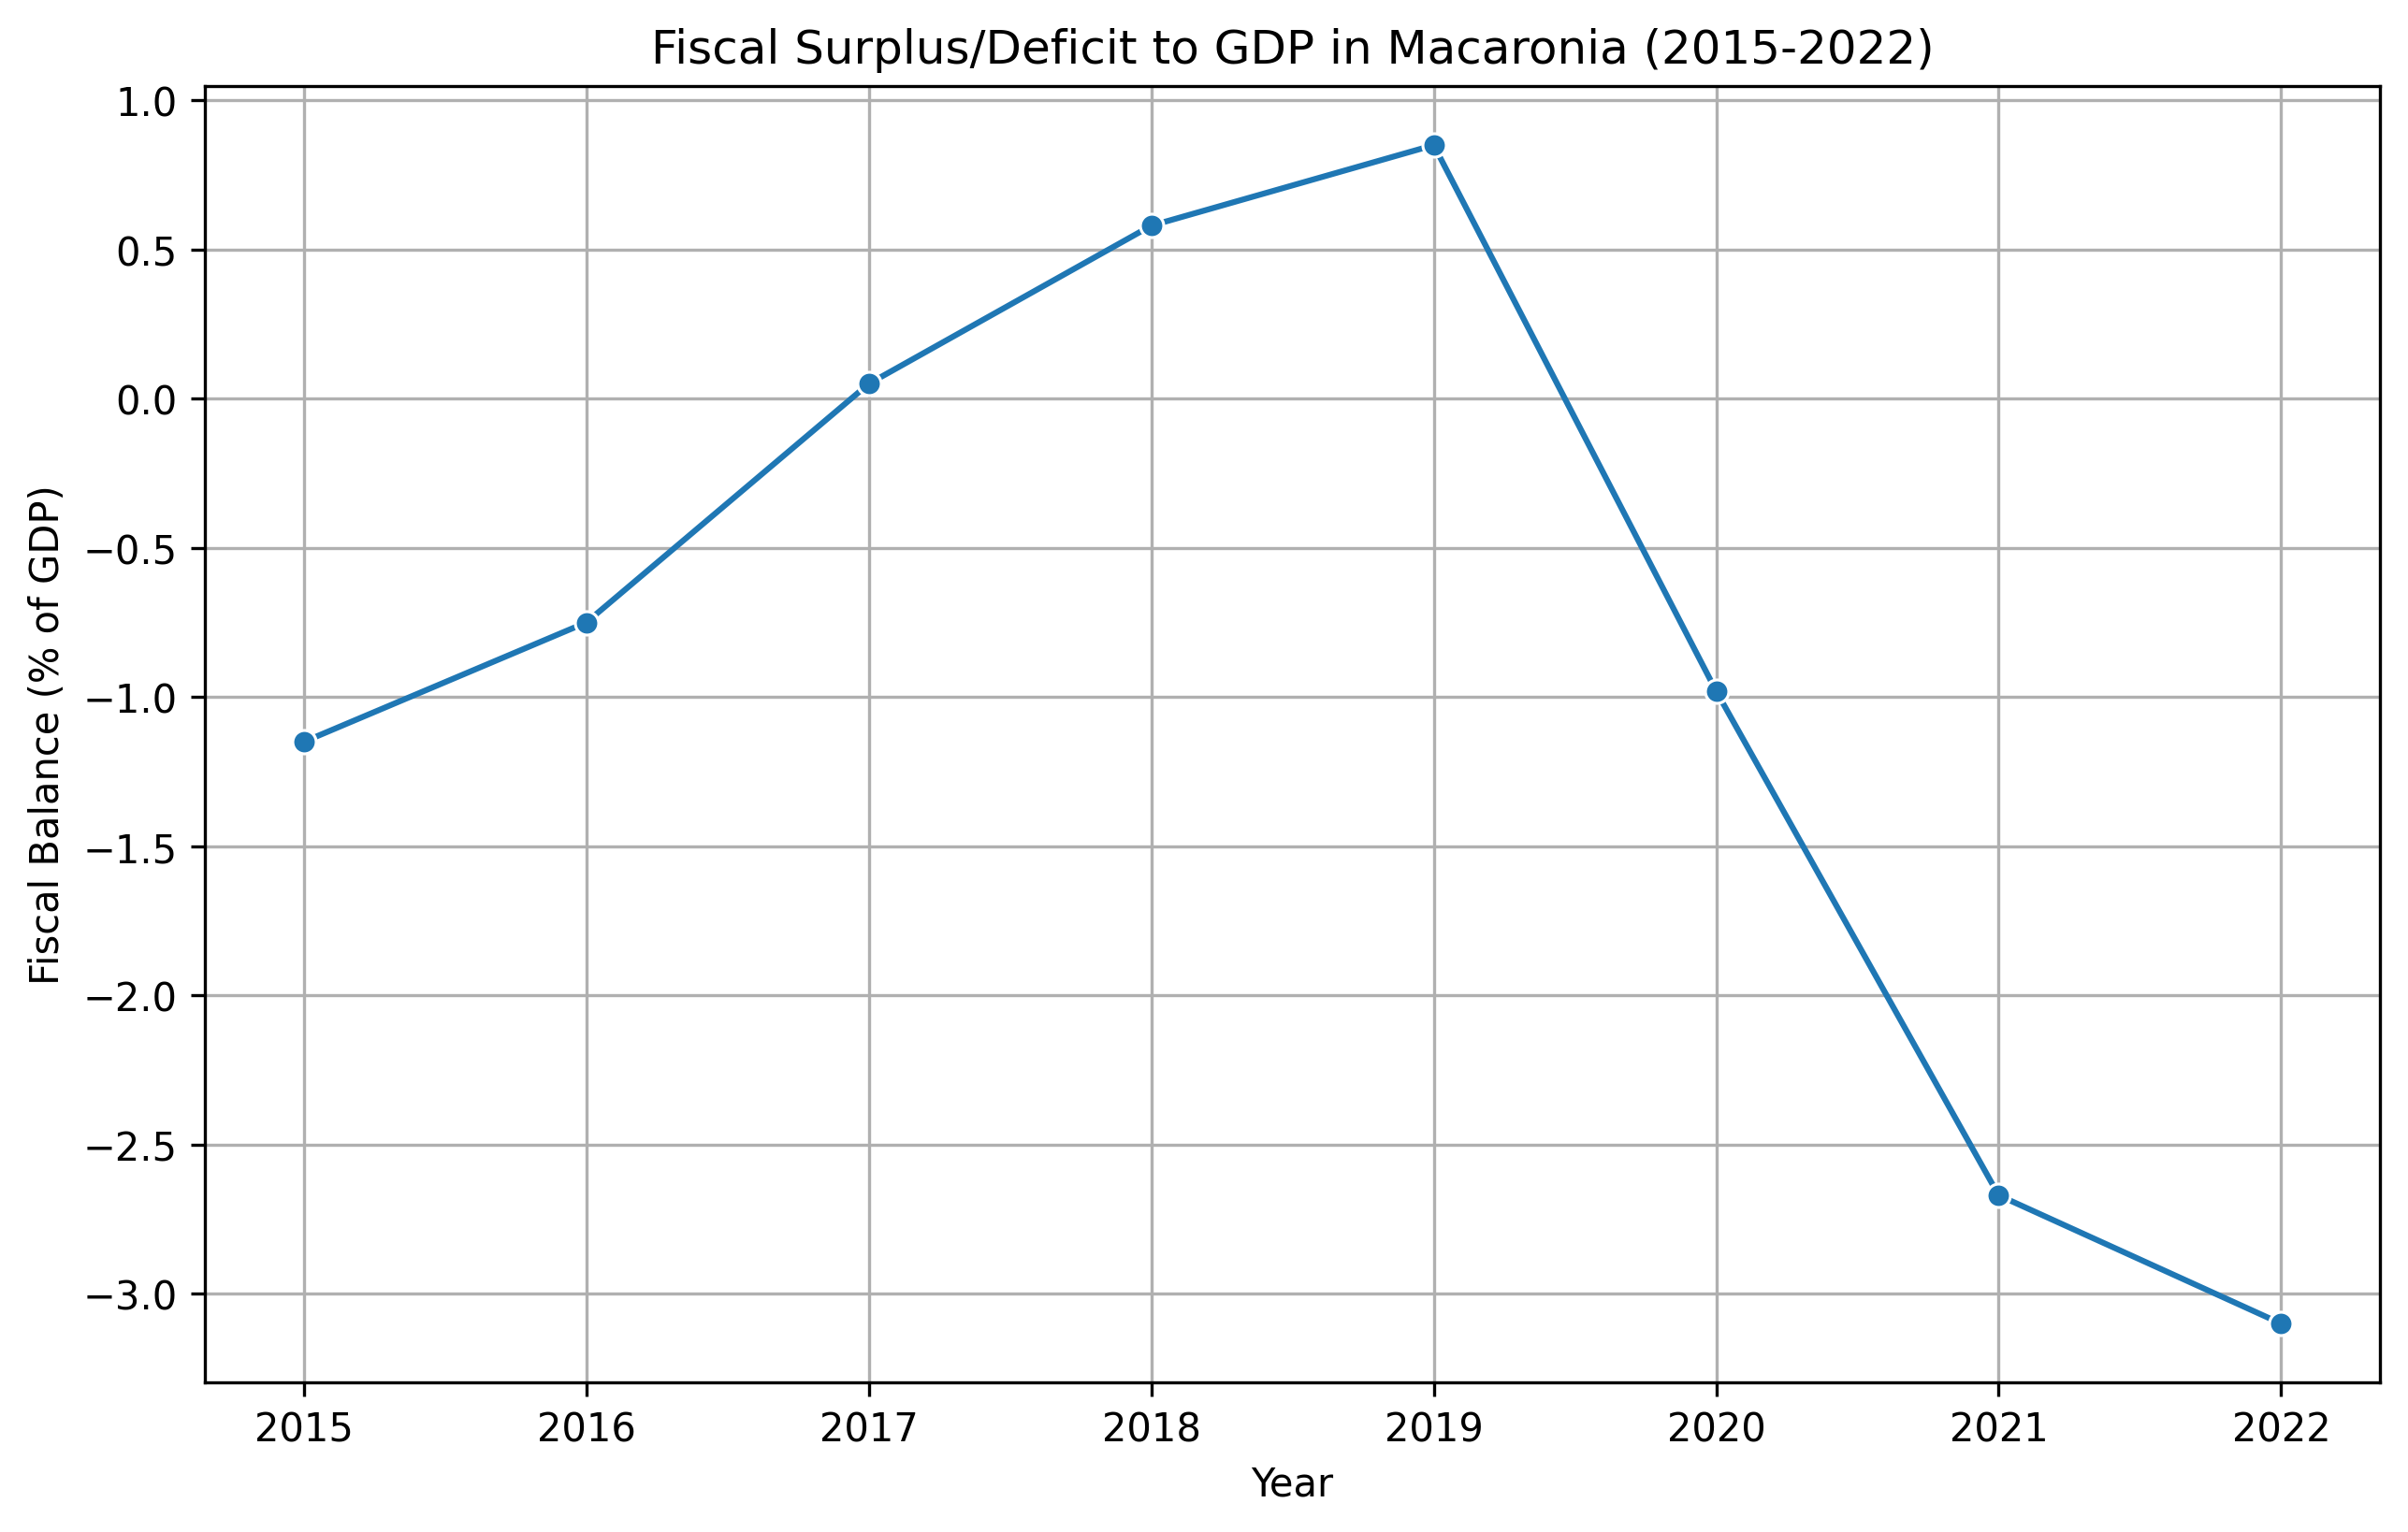
\includegraphics[width=\textwidth]{fiscal_to_gdp.png}
        \caption{\small Fiscal Surplus/Deficit to GDP in Macaronia}
        \label{fig:fiscal_to_gdp}
    \end{subfigure}
    \caption{Macaronia’s Public Debt and Fiscal Position (2015-2022)}  % Main figure caption
    \label{fig:public_debt_fiscal}
\end{figure}


As depicted in Figure 2(a), Macaronia's public sector debt has steadily increased, reaching
\textcolor{teal}{\textbf{80\% of GDP}} in 2022 from \textcolor{teal}{\textbf{68\% of GDP}} 
in 2015, reflecting a concerning trend. This trajectory indicates a growing reliance on borrowing
to finance government expenditures. Concurrently, Figure 2(b) illustrates a significant deterioration
in the fiscal position, with \textcolor{teal}{\textbf{fiscal deficits}} widening to 
\textcolor{teal}{\textbf{-3.1\% of GDP}} in 2022. This widening deficit suggests that 
government spending has outpaced revenues, contributing to the rising debt burden. 
The combination of high debt levels and persistent deficits raises serious concerns 
about the sustainability of Macaronia's fiscal position, particularly in light of tightening 
\textcolor{teal}{\textbf{global financial conditions}}.

%(Insert "Credit Extended by Banks and Credit Unions" graph here)
%(Insert "Liquidity Ratios – Banks and Credit Unions" graph here)
%(Insert "Capital Adequacy Ratios – Banks and Credit Unions" graph here)

\subsection*{Implications for Economic Theory}

\begin{enumerate}
    \item \colorbold{teal}{Moral Hazard in Financial Regulation}: The moral hazard theory states that financial
                         institutions, particularly banks and credit unions in Macaronia, have taken excessive
                         risks of overexposure to volatile REITs. They operated under the assumption that the
                         central bank would intervene in times of crisis \textcolor{orange}{\cite{holmstrom1997}}. This said
                         behaviour increases systemic risk in the economy. \textcolor{orange}{\cite{allen2015}}.

    \item \colorbold{teal}{Ricardian Equivalence and Public Debt}: The Ricardian Equivalence Theory suggests that rising 
                          public debt may lead to decreased private consumption as people foresee future tax increases.
                          In Macaronia, rising public debt could effectively shrink consumer confidence and as a result,
                          dampen economic recovery.

    \item \colorbold{teal}{Exchange Rate and Reserve Management}: Rapid depleting reserves pose a grave concern for Macaronia’s
                           central bank. According to Mundell’s (1961) theory, a floating exchange rate can repair external 
                           shocks, however, a large depletion of the reserves may force the central bank to intervene to ensure
                           the stability of its currency. \textcolor{orange}{\cite{mundell1961}}
\end{enumerate}

\subsection*{Global Financial Outlook}

% (Insert the "Global Economic Growth" graph here)
\begin{figure}[h]
     \centering
     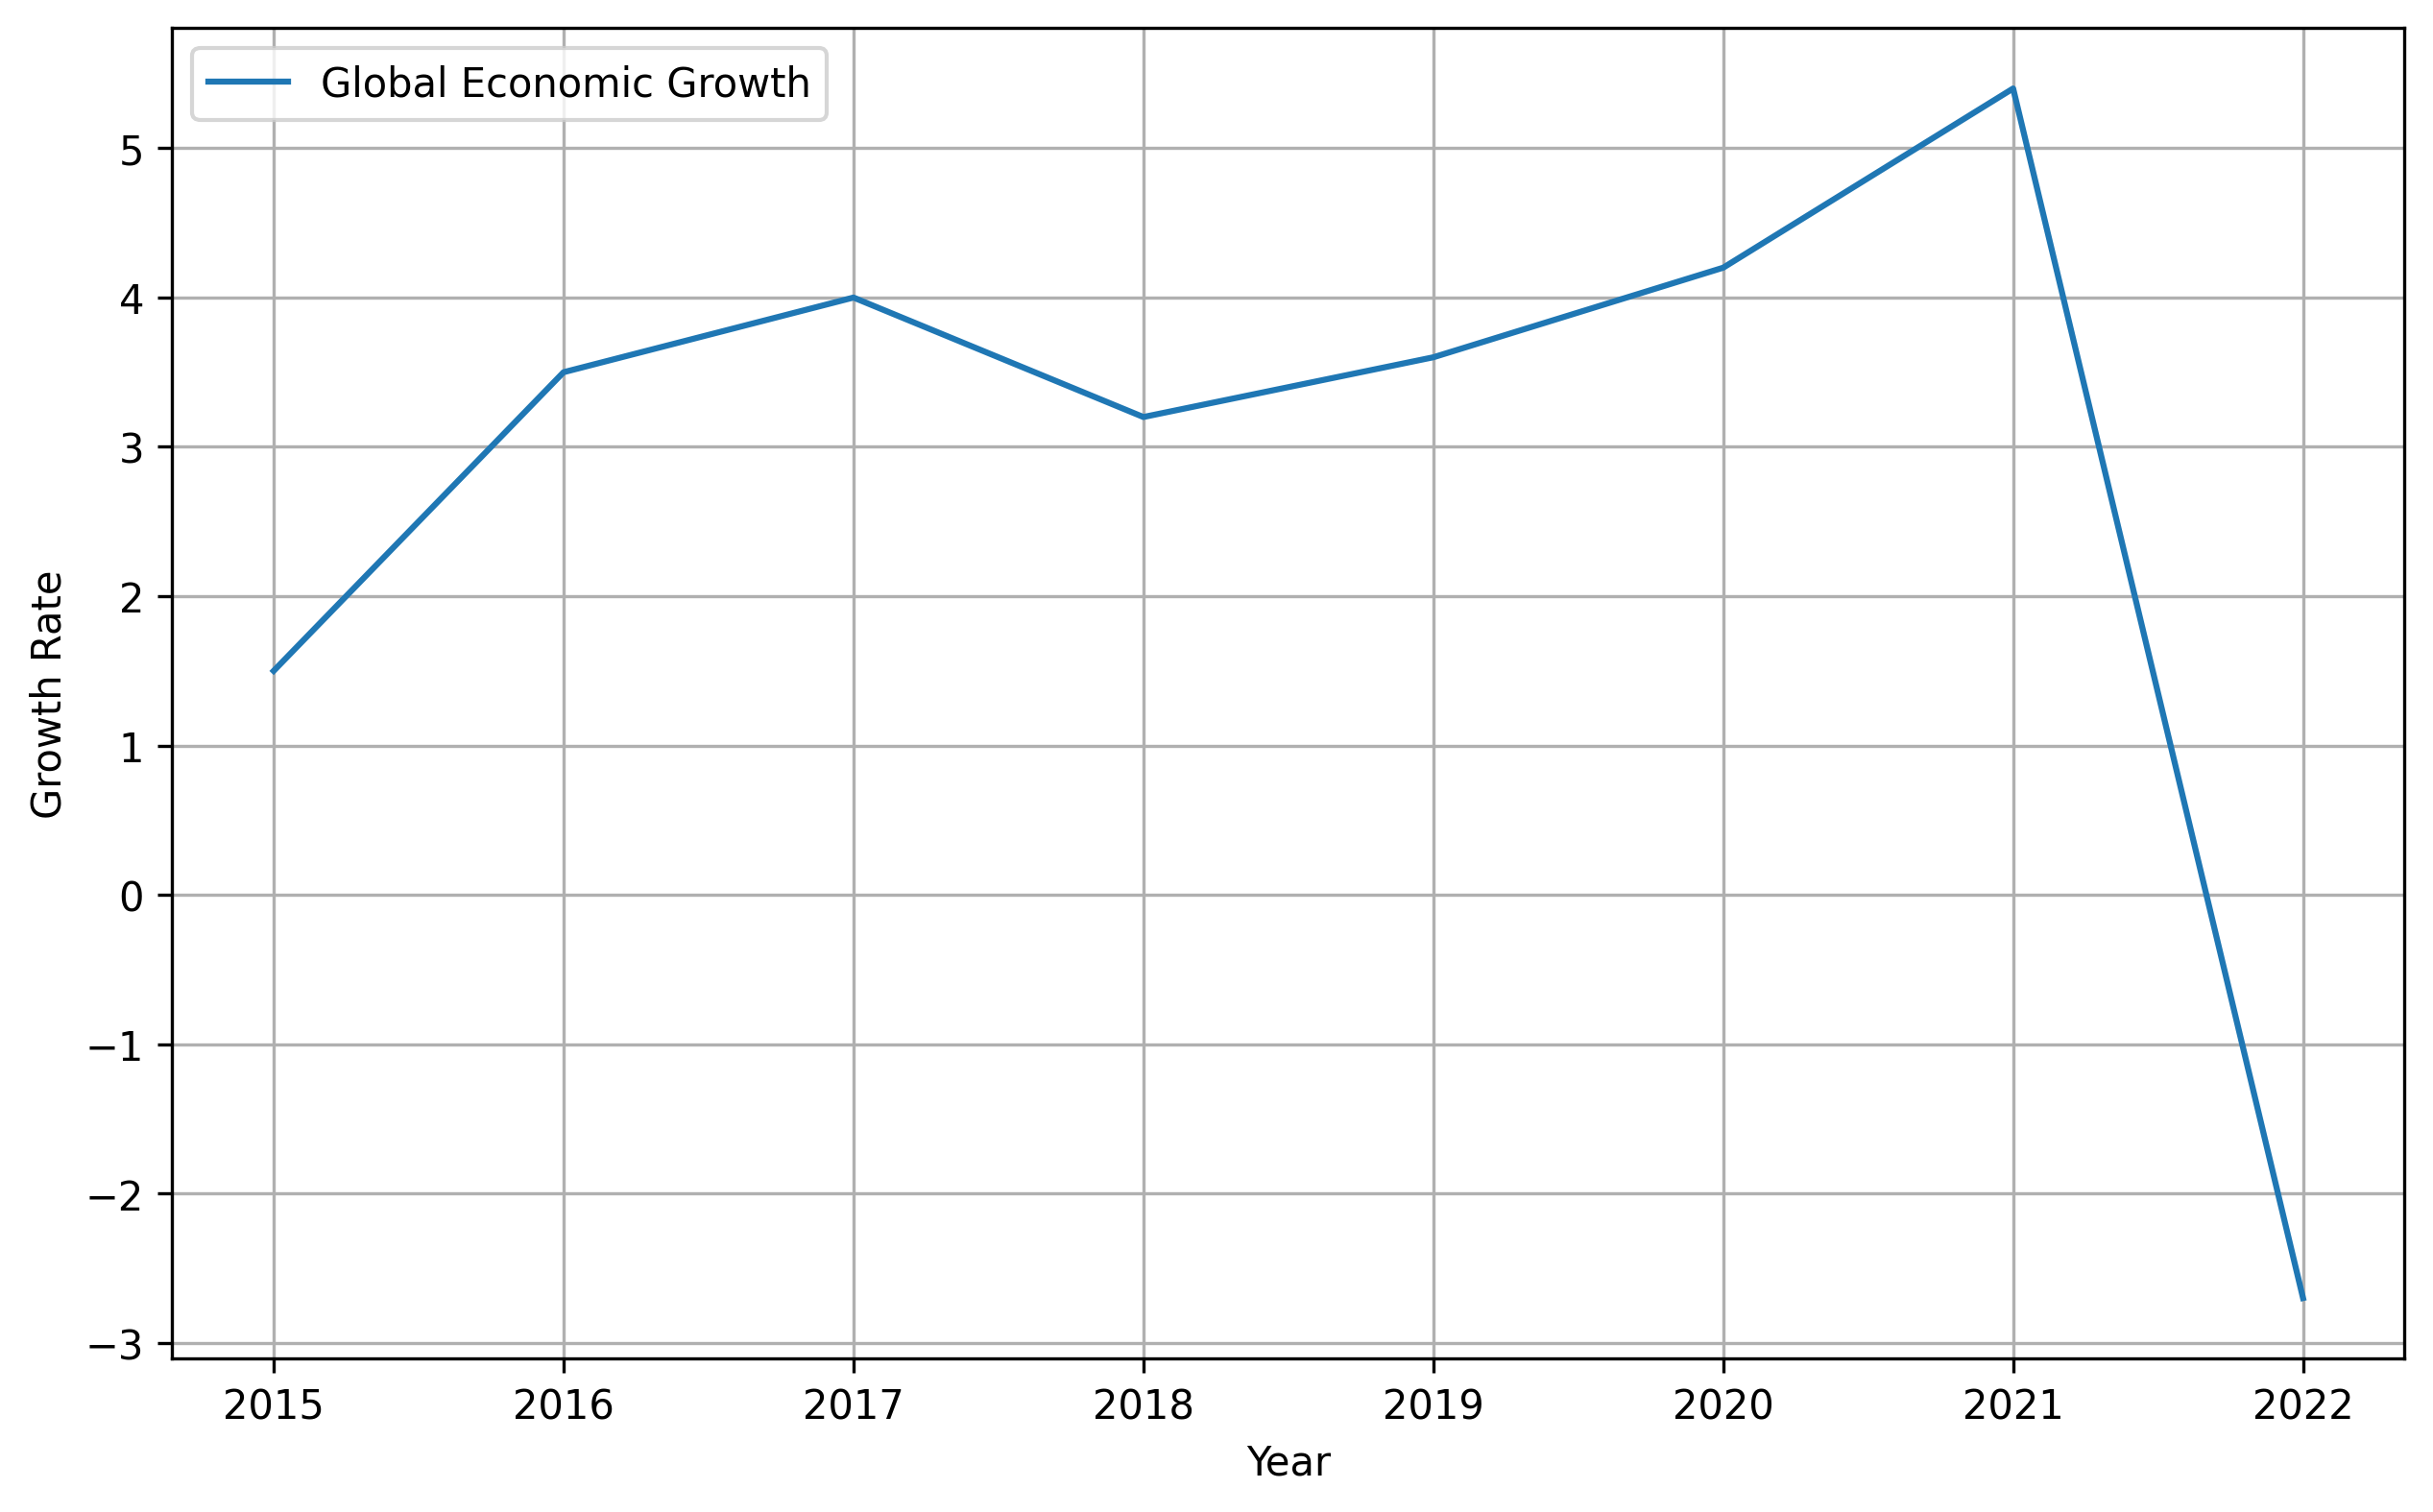
\includegraphics[width=0.6\textwidth]{growth2.png}
     \caption{Global Economic Growth}
     \label{fig:graph_1}
\end{figure}

As depicted in Figure 3, the global economy has experienced significant volatility, with severe shocks 
affecting financial stability. One such shock was due to the collapse of a major U.S. financial institution,
which led to disruptions in global credit markets and increased uncertainty.

As previously mentioned, the IMF estimates a contraction in global economic activity in 2023 by \textcolor{teal}{\textbf{2.5\%}}
and in 2024 by \textcolor{teal}{\textbf{3\%}}. These conditions raise concerns for small, open economies like
Macaronia, which are heavily bound to international financial markets. The ongoing weakening of investor
confidence continues to deplete Macaronia's international reserves due to capital flight, further straining
Macaronia's financial stability.


